\subsection{Break-even Kernel Startup Time}
We can see that the asynchronous kernel startup time stays roughly constant
until a processing time of around 3100 clock cycles, after which it starts
rising linearly with increasing clock cycles. This indicates that until 3100 cycles
the GPU spends time idle even after the kernel is finished processing. After 3100 cycles,
the next kernel can be directly launched without additional overhead. Roughly 8200 clock cycles are needed until the initial asynchronous time of around 2.7 s doubles.\\
This time of around 5.3 s consists of 2.7 s for the kernel startup time in addition to another 2.7 s coming from time only spent processing.\\
In this time (5.3 s or 8200 clock cycles), another kernel launch call could have been completed.
\begin{figure}
    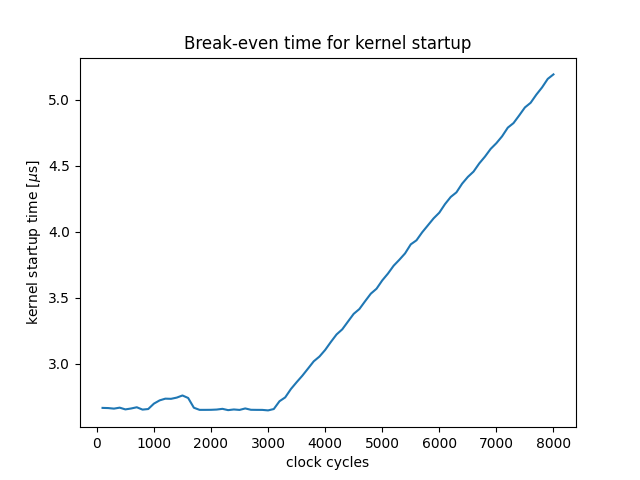
\includegraphics[scale=0.7]{break-even.png}
    \caption{exercise 2.2, break-even kernel startup time}
    \label{fig:202BreakEven}
\end{figure}
